\documentclass[11pt]{article}
\usepackage[utf8]{inputenc}
\usepackage{mathtools}
\usepackage{vmargin}
\usepackage{graphicx}
\usepackage{lmodern}
\usepackage[T1]{fontenc}
\usepackage{multirow}
\usepackage[noline,ruled,linesnumbered,spanish]{algorithm2e}
\usepackage{forest}
\usepackage{forest,adjustbox}
\usepackage{color}

\setpapersize{A4}
\setmargins{2.5cm}       % margen izquierdo
{0cm}                        % margen superior
{16.5cm}                      % anchura del texto
{23.42cm}                    % altura del texto
{10pt}                           % altura de los encabezados
{1cm}                           % espacio entre el texto y los encabezados
{0pt}                             % altura del pie de página
{2cm}                           % espacio entre el texto y el pie de página

\title{Mini-Proyecto III: Estructuras de Datos Sucintas}
\author{Cristobal Donoso Oliva}
\author{
Diego Seco$^{1}$, Meraioth Ulloa Salazar$^{2}$, Cristóbal Donoso Oliva$^{3}$,\\ Matías Medina Silva$^{4}$,\\ \\
\small{$^{1}$Docente a cargo de la asignatura$^{2-3-4}$Estudiantes Pre-grado}\\
\small{$^{1-2}$Dpto. de Ingeniería Civil Informática y Ciencias de la Computación}\\
\small{Universidad de Concepción, Concepción, Chile.}\\
}
\date{Noviembre de 2016}
\usepackage{amsmath}
\begin{document}

\maketitle

\section{Range Minimum Query}
\subsection{Descripción del Problema}
El problema de RMQ (Range Minimum Query) consiste en encontrar el mínimo dentro de un rango [i,j] perteneciente a un arreglo de n objetos que se pueden comparar. En particular, resolveremos el problema para un arreglo de números. Usualmente debemos resolver RMQ en el desarrollo de otros problemas, tales como: Lowest Common Ancestors o del áres de Document Retrieval.\\\\En la práctica existen varias soluciones candidatas a este problema, sin embargo, no todas ellas rinden de igual manera. Con el objetivo de comparar experimentalmente la complejidad asociada al RMQ, utilizaremos dos alternativas antagonistas de solución.\\
\begin{center}\begin{tabular}{|c|c|c|c|c|c|c|}
\hline
	13 & 2 & 7 & 0 & 9 & 10 & 27 \\
\hline
\end{tabular}
\\\scriptsize{\color{white}.\color{black}\\Figura 1: Data set con números}
\end{center}
Sea $RMQ$ la función que retorna el minimo del rango $[i,j]$, con 0$\le$i$\le$ j$\le$n, entonces: \begin{center}$RMQ[2,6] = 0$\\$RMQ[0,2] = 2$\\$RMQ[4,4] = 9$\end{center}  
\subsection{Solución Naive}
Consiste en almacenar los mínimos asociados a todas las sub-cadenas que pertenecen al arreglo de números; con esto realizamos consultas en tiempo $O(1)$, sin embargo, la complejidad espacial asciende a $O(n^2)$. Cabe mencionar que en situaciones donde \emph{el recurso espacial no es relevante}, implementar esta solución es una alternativa rápida y sencilla a la hora de computar las consultas, sin embargo, es importante añadir que los datos consultados deben cumplir la condición de \emph{ser estáticos}, en su defecto, el dinamismo actualizaría la tabla frecuentemente aumentando el tiempo de pre-procesamiento.\\\\A continuación se muestra la matriz resultante del set de números propuesto anteriormente(ver figura 1).
\begin{center}$\begin{vmatrix}
	13 & 2 & 2 & 0 & 0 & 0 & 0 \\
	 & 2 & 2 & 0 & 0 & 0 & 0 \\
	 &  & 7 & 0 & 0 & 0 & 0 \\
	 &  &  & 0 & 0 & 0 & 0 \\
	 &  &  &  & 9 & 9 & 9 \\
	 &  &  &  &  & 10 & 27 \\
	 &  &  &  &  &  & 27 \\
\end{vmatrix}$
\\\scriptsize{\color{white}.\color{black}\\Figura 2: Matriz que guarda los mínimos parciales de todos los rangos de un conjunto de números}
\end{center}
Una consulta simple bastaría con preguntar por la dirección $<i,j>$ de la matriz generada.

\subsection{Solución RMQ + Sparse Table}
Podemos resolver el problema RMQ optimizando la matriz que almacena los mínimos utilizando potencias de dos para definir la dimensión de la tabla (sparse table). Esta alternativa nos permite disminuir el espacio realizando consultas en tiempo constante. En efecto, las complejidades asociadas al espacio y consulta son $O(nlog(n))$ y $O(1)$ respectivamente.\\\\La cantidad de filas corresponden a los datos en el set, sin embargo, las columnas responden a $O(log(n))$. La idea consiste en pre-computar el mínimo de todas las sub-cadenas de tamaño $2^k$ donde $0 \le k \le log(n)$. Del mismo set (figura 1) la tabla generada es:

\begin{center}$\begin{vmatrix}
	0 & 1 & 3   \\
	1 & 1 & 3   \\
	2 & 3 & 3   \\
	3 & 3 &     \\
	4 & 4 &     \\
	5 & 5 &     \\
	6 &   &	    \\
\end{vmatrix}$
\\\scriptsize{\color{white}.\color{black}\\Figura 2: Sparse Table para el set}
\end{center}
Para calcular la tabla es necesario saber la cantidad de columnas $j$ que tendrá la tabla, para ello calculamos:
\begin{center}$\#j$ = log(\emph{$\#$ elementos})  $\iff \lfloor log(7) \rfloor+1 \iff 2 +1 = 3$
\end{center}
Donde $\#$ representa la cardinalidad y $log$ es de base 2. Luego buscamos los mínimos que se encuentran dentro de los rangos $2^j$ con $0\le j \le 2$ para cada posición $i$. Para realizar la consulta debemos comparar:
\begin{center}$arr[lookup[i][j-1]]$ $\nabla$ $arr[lookup[i+2^j-1-1][j-1]]$\end{center}
Donde $\nabla$ = $\{\le,\geq\}$. RMQ retorna el menor entre los valores comparados. 

\subsection{Experimento}
Anteriormente determinamos teóricamente la complejidad espacial de los dos algoritmos en cuestión. Es fácil demostrar en la práctica como influye la construcción de las tablas ya que éstas alteran la tiempo de ejecución en directa proporción con la cantidad de elementos. En ese sentido, al realizar consultas bajo \emph{datasets} dinámicos, la segunda alternativa tendrá mejor rendimiento.\\\\Para los \emph{sets aleatorios} de tamaño $10^i$ con 0<i<$10^7$ y rango $[0,random(0...i)]$ se obtuvieron los siguientes resultados:
\begin{center}\begin{tabular}{|l|c|c|}
\hline
	$Tamaño$ & $Naive$ & $Sparse$\\
\hline
	10 & 7.7e-5 & 4.4e-5\\
\hline
	100 & 0.002429 & 0.000441\\
\hline
	1000 & 0.097398 & 0.004381\\
\hline
	10000 & 8.8443 & 0.031585\\
\hline
	100000 & killed & 0.0323302\\
\hline
	1000000 & killed & 3.63675\\
\hline
	10000000 & killed & 40.3935\\
\hline
\end{tabular}
\\\scriptsize{\color{white}.\color{black}\\Figura 3: Tabla de resultados tiempo de ejecución algoritmos propuestos}
\end{center}
Para mayor claridad solo se muestra el gráfico hasta i = 800
\begin{center}\begin{figure}[htp]
\centering
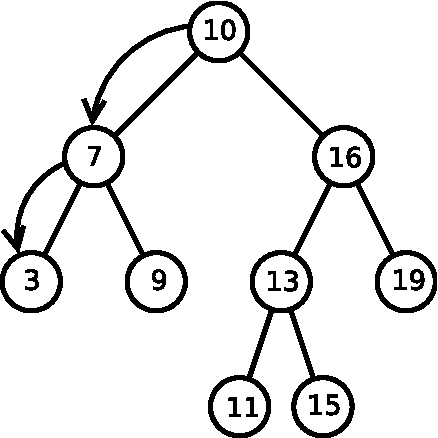
\includegraphics[scale=0.5]{min_arbol.pdf}
\\\scriptsize{\color{white}.\color{black}\\Figura 4: Bifurcación que muestra las diferencias en tiempo de ejecución de los algoritmos naive y sparse}
\label{etiqueta}
\end{figure}
\end{center}
\clearpage
\section{predecesor y sucesor}
\subsection{Descripción del problema}
Se tiene \textbf{t} elementos de un conjunto [1,n] y se quieren hacer dos tipos de consultas sobre dicho conjunto:
\begin{itemize}
\item Sucesor: Dado un número i, ¿Cuál es el menor número $\geq$ i en el conjunto?
\item Predecesor: Dado un número i, ¿Cuál es el mayor número $\leq$ i en el conjunto?
\end{itemize}
Para este problema se proponen dos soluciones usando las siguientes estructuras de datos:
\subsection{Solución BST}
Para poder calcular el predecesor y sucesor de un elemento del BST primero debemos definir el mínimo y máximo elemento en un árbol binario. Los nodos mínimo y máximo de un BST se encontrarían más a la izquierda y más a la derecha respectivamente desde la raíz (ver figura 5 y 6). 
\begin{figure}[htp]
\centering
\begin{minipage}{.4\textwidth}
\centering
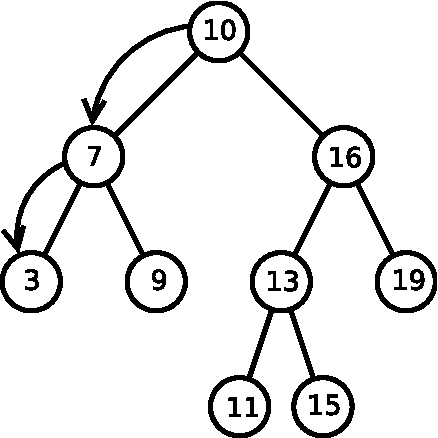
\includegraphics[scale=0.5]{min_arbol.pdf}
\\\scriptsize{\color{white}.\color{black}\\Figura 5: Nodo mínimo en un BST}
\label{etiqueta}
\end{minipage}
\begin{minipage}{.4\textwidth}
\centering
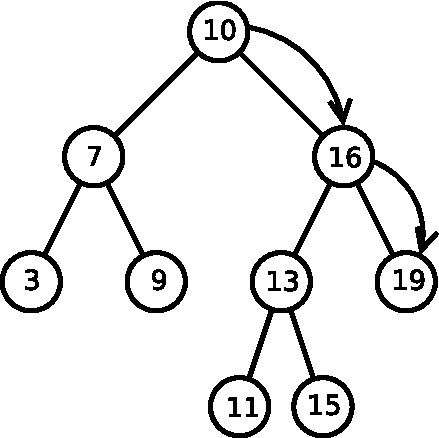
\includegraphics[scale=0.5]{max_arbol.pdf}
\\\scriptsize{\color{white}.\color{black}\\Figura 6: Nodo máxmimo en un BST}
\label{etiqueta}
\end{minipage}
\end{figure}

Entonces, Para poder encontrar el predecesor y sucesor:
\begin{itemize}
\item Si el nodo i tiene dos hijos su predecesor es el valor máximo en el sub-árbol a la izquierda de i y su sucesor sería el valor mínimo en en el sub-árbol a la derecha de i.
\item Si no entonces:
\begin{itemize}
\item Si i no tiene hijo izquierdo entonces su predecesor es su primer ancestro izquierdo.
\item Si i no tiene hijo derecho entonces su sucesor es su primer ancestro derecho.
\end{itemize}
\end{itemize}
\subsection{Solución Bitmap}
Cada indice del bitmap B representa un elemento de conjunto [1,n], donde un 1 representa que el elemento es uno de los t elementos, como se puede ver en la figura 7.\\

\begin{figure}[htp]
\centering
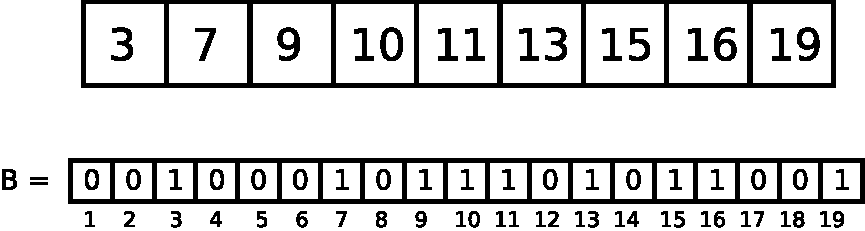
\includegraphics[scale=0.5]{bitmap.pdf}
\\\scriptsize{\color{white}.\color{black}\\Figura 7: Nodo mínimo en un BST}
\end{figure}
Para responder a las consultas predecesor y sucesor podemos usar las operaciones rank y select de los bitmaps:
\begin{itemize}
\item Sucesor: Select(B, Rank (B, i) + 1)
\begin{figure}[htp]
\centering
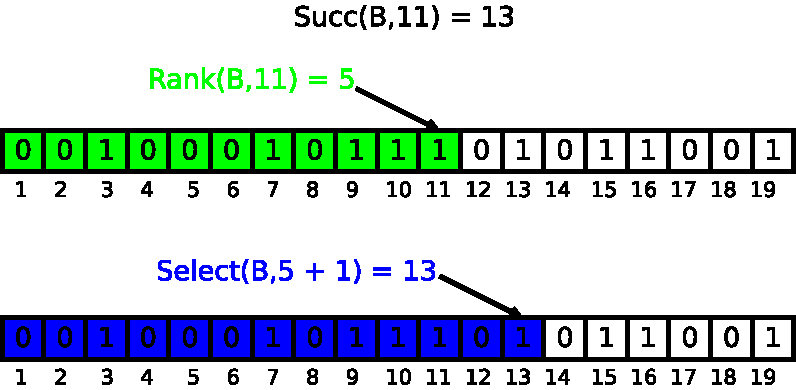
\includegraphics[scale=0.5]{bitmapsuc.pdf}
\\\scriptsize{\color{white}.\color{black}\\Figura 8: Ejemplo de sucesor con i = 11}
\end{figure}
\item Predecesor: Select(B, Rank (B, i $-$ 1))
\begin{figure}[htp]
\centering
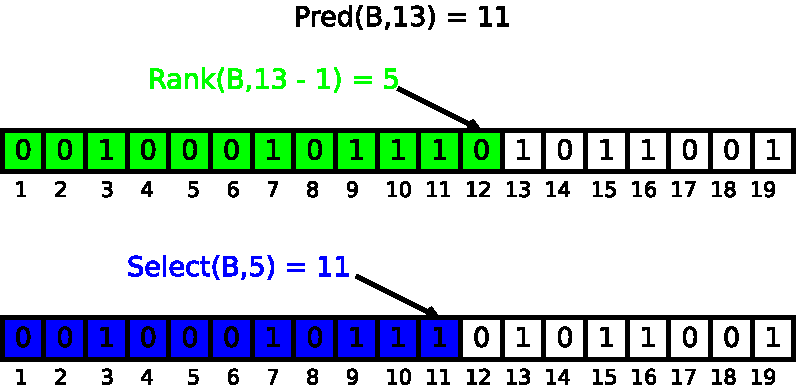
\includegraphics[scale=0.5]{bitmappred.pdf}
\\\scriptsize{\color{white}.\color{black}\\Figura 9: Ejemplo de predecesor con i = 11}
\end{figure}
\end{itemize}
\subsection{Análisis de complejidad de las soluciones}
\subsubsection{BST}
Las operaciones necesarias para obtener el predecesor y sucesor toman un tiempo que es proporcional a la altura del árbol. Para un BST con n nodos, las operaciones quedan acotadas a tiempos O(Log(n)) usando el método de analsis en el caso promedio y acotadas a tiempos O(n) usando el método de peor caso, cuando el árbol no está balanceado y hay que recorrer los nodos de manera secuencual.
\subsubsection{Bitmap}
Las únicas operaciones utilizadas en el bitmap son rank y select, las cuales pueden ser respondidas en tiempo constante O(1) utilizando bitmaps normales y también en tiempo O(k) para rank (k es la clave) y O(log n)  para select utilizando bitmaps H$_{0}$ - comprimidos, ambos ya implementados en la librería sdsl.

\end{document}
